\hypertarget{qmanagerelation_8cpp}{}\section{O\+L13/qmanagerelation.cpp File Reference}
\label{qmanagerelation_8cpp}\index{O\+L13/qmanagerelation.\+cpp@{O\+L13/qmanagerelation.\+cpp}}


Fenetre de dialoque permettant de gérer les relations.  


{\ttfamily \#include \char`\"{}qmanagerelation.\+h\char`\"{}}\newline
{\ttfamily \#include \char`\"{}ui\+\_\+qmanagerelation.\+h\char`\"{}}\newline
Include dependency graph for qmanagerelation.\+cpp\+:\nopagebreak
\begin{figure}[H]
\begin{center}
\leavevmode
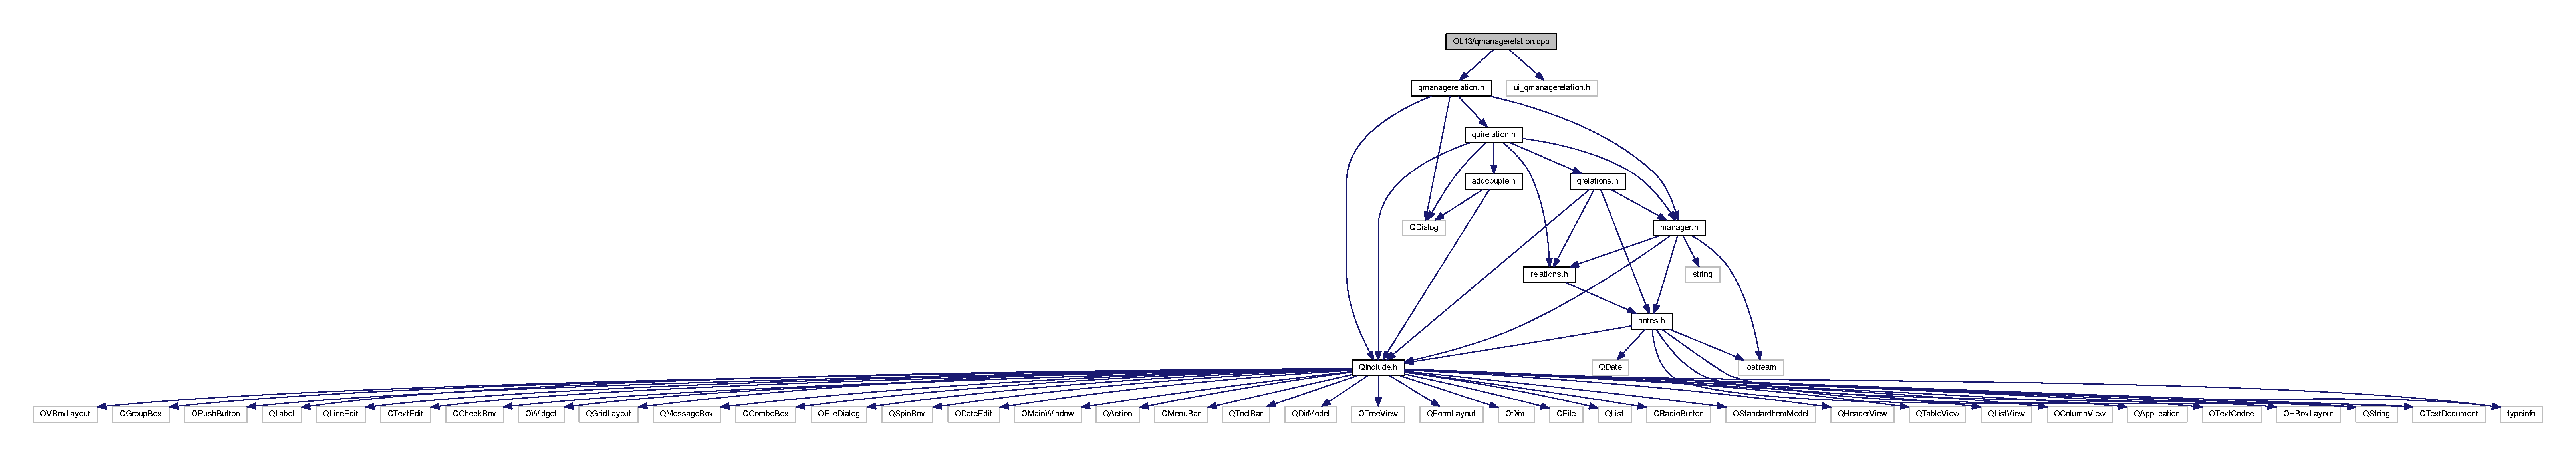
\includegraphics[width=350pt]{qmanagerelation_8cpp__incl}
\end{center}
\end{figure}


\subsection{Detailed Description}
Fenetre de dialoque permettant de gérer les relations. 

\begin{DoxyAuthor}{Author}
Garnier Maxime, Naudin Louise, Pépin Hugues 
\end{DoxyAuthor}
\begin{DoxyVersion}{Version}
1.\+0 
\end{DoxyVersion}
\begin{DoxyDate}{Date}
14 Juin 2017
\end{DoxyDate}
attributs \+: Q\+String currentR // titre de la relations selectionné Signaux\+: void update\+\_\+relation() 